% arara: pdflatexmk: { synctex: "--synctex=1" }

\documentclass[%
	shownavigationbar=	false,%
	showsidebar= 		false,%
	fleqn,%
	xcolor=				{usenames, svgnames},%
	usepdftitle=		false,%
%	compress,%
%	draft,%
]{beamer}

\usepackage{%
	marvosym,%
	graphicx,%
	hyperref,%
	parskip,%
	booktabs,%
	tabularx,%
	multicol,%
	microtype,%
%	etex,%
	array,%
	colortbl,%
	xspace,%
	enumerate,%
	amsmath,%
}

\definecolor{VUBlue1}{cmyk}{1,0,0,0}
\definecolor{VUBlue2}{cmyk}{1,0.16,0,0.20}
\definecolor{VUBlue3}{cmyk}{1,0.55,0,0.18}
\definecolor{FEWEB1}{cmyk}{0.60,0.90,0,0}
\definecolor{FEWEB2}{cmyk}{0.5,1,0,0}
\definecolor{FEWEB3}{cmyk}{0.30,0.90,0,0}
\definecolor{Ivory2}{rgb}{0.93,0.93,0.88}
\definecolor{Ivory3}{rgb}{0.8,0.8,0.76}

\usepackage{tikz}
\usetikzlibrary{positioning, backgrounds, fit, arrows.meta, calc}% fit, backgrounds,arrows.meta,

\newcommand{\link}[2]{\tikz[baseline=-2pt]\node[rectangle, inner sep=2pt, rounded corners=.75pt, draw=VUBlue3] {\href{#1}{\texttt{#2}}};\xspace}

\newcommand{\bula}{{\tikz\node[rectangle, inner sep=2pt, rounded corners=.75pt, draw=VUBlue3, thick, fill=VUBlue3] {};}\xspace}%fill=VUBlue1!75
\newcommand{\bulb}{\tikz\node[rectangle, inner sep=2pt, rounded corners=.75pt, draw=VUBlue3, thick] {};\xspace}
\newcommand{\bulc}{\tikz\draw[VUBlue3, thick] (0,0) (0,.3ex)--(5pt,.3ex) (.6em,0);\xspace}%(0,.75ex)--(.6em,.75ex)

\usepackage{enumitem}%
\setlist[itemize,1]{label={\raisebox{0.2ex}\bula}, itemsep=.5ex, topsep=1ex}%
% LEVEL 2
\setlist[itemize,2]{label={\raisebox{0.2ex}\bulb}, itemsep=.5ex, topsep=.75ex}%
% LEVEL 3
\setlist[itemize,3]{label=\bulc, itemsep=.25ex, topsep=.5ex}%

\usepackage[T1]{fontenc}

\usepackage[UKenglish]{babel}

\usetheme{default}
\mode<presentation>
\usecolortheme{default}
\usecolortheme{rose}
\setbeamercovered{transparent=30}

\setbeamercolor{structure}{fg=VUBlue3} % titlelike
\setbeamercolor{normal text}{fg=black}
\setbeamercolor{alerted text}{fg=FEWEB2}

\setbeamertemplate{subsection in toc}{%
	\leavevmode\leftskip=5.65ex%
	\llap{\raisebox{0.3ex}{{\bulc}}\kern1ex}%
  	\inserttocsubsection\par%
}
\setbeamertemplate{subsection in toc shaded}[default][0]%
\setbeamertemplate{title page}[default][left]%
\setbeamertemplate{navigation symbols}{}%
\setbeamertemplate{blocks}[rounded][shadow=false]
%\setbeamercolor{block title}{bg=VUBlue2!5, fg=white}%
\setbeamercolor{block title}{bg=white, fg=VUBlue3}%
%\setbeamercolor{block body}{bg=VUBlue2!5, fg=black}%
\setbeamercolor{block body}{bg=white, fg=black}%
\setbeamercolor{block title alerted}{bg=FEWEB1, fg=white}%
\setbeamercolor{block body alerted}{bg=FEWEB2!10, fg=black}%
\newcommand{\plus}{\textcolor{Green}{$+$}\ }
\newcommand{\minus}{\textcolor{Red}{$-$}\ }

%%%%
\title{Finding information}
\author{Matthijs de Zwaan}%

\date{1 November 2017}

\begin{document}
\section{Front matter}
% TITLE PAGE
\begin{frame}<1>[plain, label=titlepage]
\begin{tikzpicture}[remember picture,overlay]
	\node[anchor=center, at={(current page.center)}] {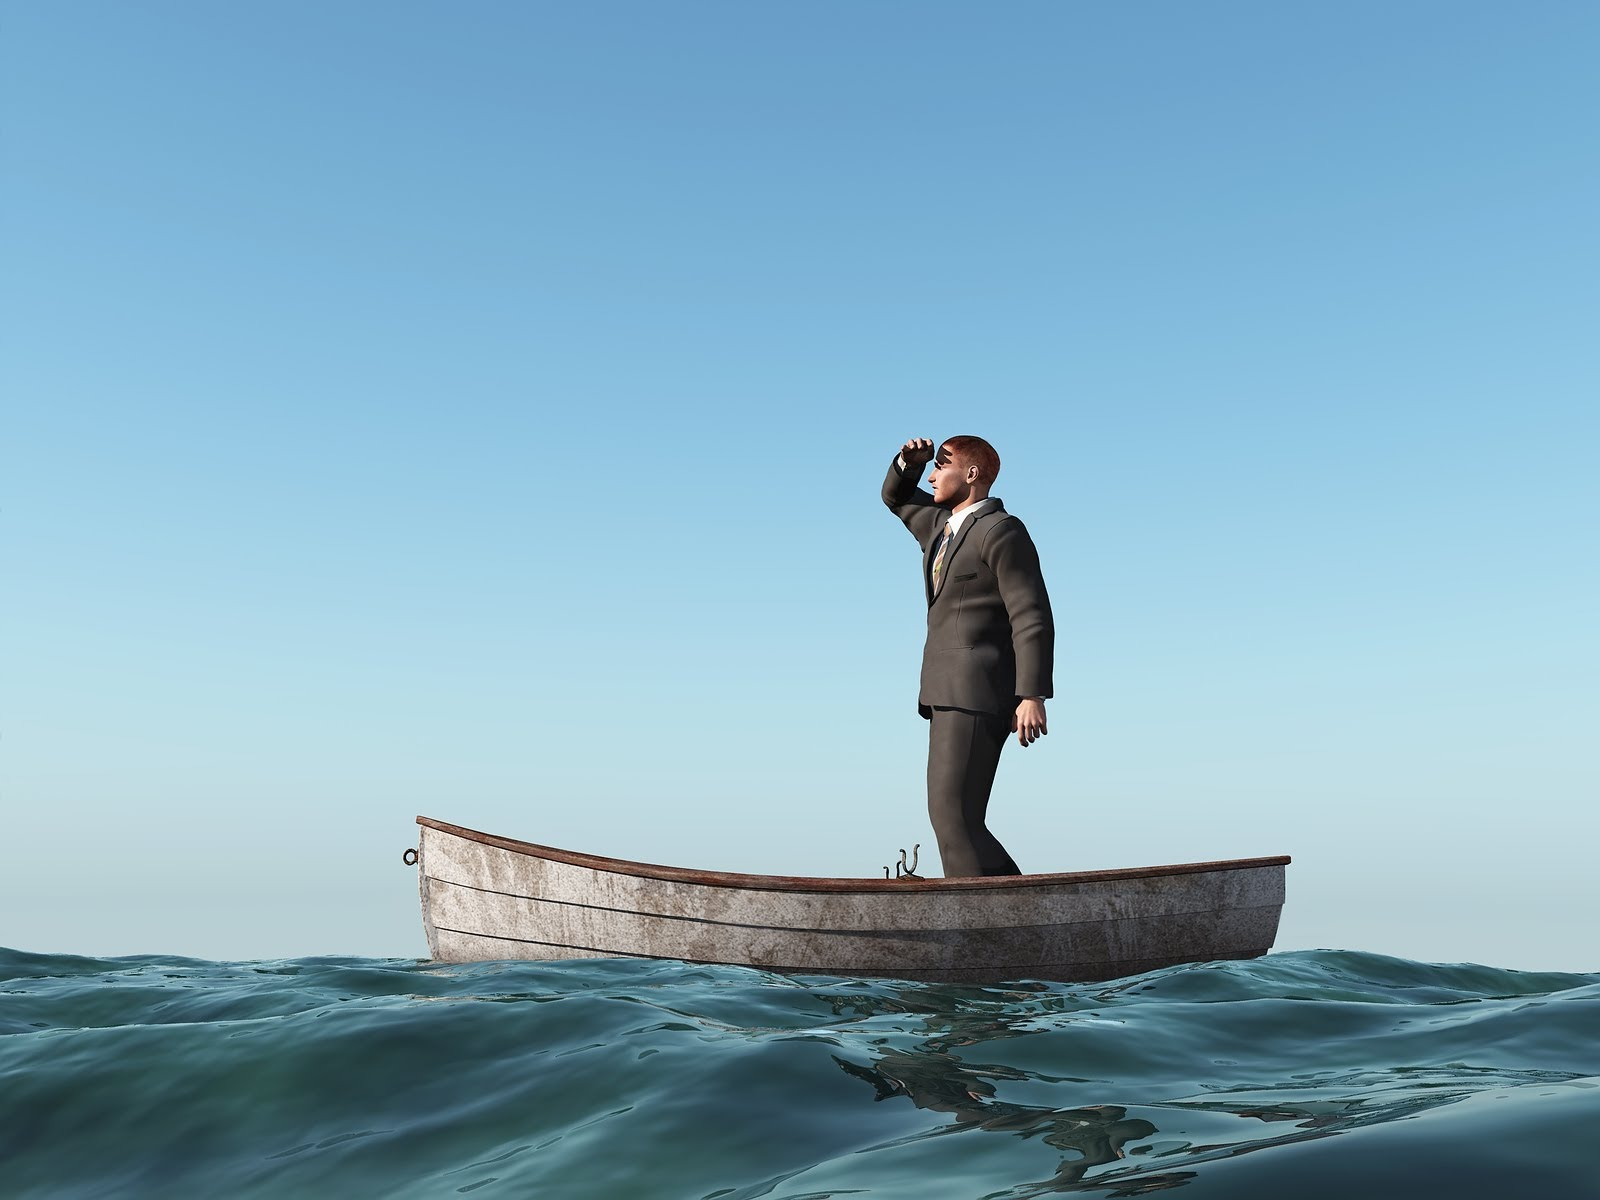
\includegraphics[width=\paperwidth]{lost-at-sea}};
\end{tikzpicture}
\only<1>{
\begin{tikzpicture}[align=left, inner sep=0pt, overlay, anchor=west]
	\node (title) [text width=6cm] at (0pt,1cm) {\Large\bfseries Finding information};
	\node (author) [text width=6cm, below={3ex of title}] {\large\bfseries Matthijs de Zwaan};
	\node[text width=6cm, below={1ex of author}] {\bfseries\url{m.c.de.zwaan@vu.nl}};
\end{tikzpicture}
}
\end{frame}

% Object/Preview
\begin{frame}<1,2>[label=preview]
\frametitle{Stages in the thesis trajectory}
\begin{columns}[t]
\column{.2\textwidth}
\column{.8\textwidth}
\vskip 2ex
\uncover<1,2>{
	{\only{\color{VUBlue3}}<2>Developing a research question}\\
	\textcolor{black!60}{Get to know your topic}\\
	\textcolor{black!60}{Mapping the academic debate}
}
\vskip 3ex
\uncover<1,3>{
	{\only{\color{VUBlue3}}<3>Answering your research question}\\
	\textcolor{black!60}{Finding research data}
}
\vskip 3ex
\uncover<1,4>{
	{\only{\color{VUBlue3}}<4>Communicating your answer}\\
	\textcolor{black!60}{Formatting your bibliography}
}
\end{columns}
\end{frame}

\section{Developing a research question}

\begin{frame}
\frametitle{Developing a research question}
\tikzstyle{every picture}+=[remember picture, overlay]
\begin{columns}[t]
\column{.2\textwidth}
\column{.8\textwidth}
%{\color{VUBlue3}{\tikz\coordinate (a); Get to know the field\tikz\coordinate (b);}}\\
{\color{VUBlue3}{Get to know the field}}\\
Main debates \& schools of thought\\
Recent public \& academic discussions\\
Terminology
\vskip 3ex
%{\color{VUBlue3}{\tikz\coordinate (c); Mapping the academic debate\tikz\coordinate (d);}}\\
{\color{VUBlue3}{Mapping the academic debate}}\\
What is already known?\\
How can you contribute?
\end{columns}
%\only<2>{
%	\begin{tikzpicture}
%	\node at (a) {A};
%	\path[black, thick] (a) edge (c);
%	\draw (b)--(d);
%	\end{tikzpicture}
%}
\end{frame}

\begin{frame}
\frametitle{How to search: ``Boolean search''}
{\color{VUBlue3}Search using keywords}
\begin{itemize}
\item Boolean operators: `AND' or `OR' (see \link{http://images.webofknowledge.com/WOK46/help/WOS/ht_operators.html}{here} or \link{https://youtu.be/5K_yUMvt_nU}{here}),\\[2ex]
\begin{columns}
\column{.1\linewidth}
\column{.4\linewidth}
\bulb $x\text{ AND }y$:
\begin{tikzpicture}[baseline=-1mm]
	\begin{scope}[thick]
		\draw[clip] (0,0) circle[radius=4mm];
		\node at (2.5mm,0) [fill=VUBlue2, shape=circle, minimum size=8mm, inner sep=0pt] {};
	\end{scope}
	\node at (2.5mm,0) [shape=circle, minimum size=8mm, inner sep=0pt, draw=black] {};
	\node at (-1.6mm,0){$ \scriptstyle x$};
	\node at (4.1mm,0){$\scriptstyle y$};
\end{tikzpicture}% (0.3,0) circle (.5cm);
\column{.4\linewidth}
\bulb $x\text{ OR }y$: \tikz[baseline=-1mm] \draw[fill=VUBlue2] (0,0) circle[radius=4mm] (2.5mm,0) circle[radius=4mm];% (0.3,0) circle (.5cm);
\column{.1\linewidth}
\end{columns}
\item Also useful:\\
\begin{tikzpicture}[anchor=west]
	\node at (1em,0) {\bulb parentheses: (\ldots)};
	\node at (1em,-3ex) {\bulb quotes: \textquotedbl\ldots\textquotedbl};
	\node at (13em,0) {\bulb wildcards: `*', `?'};
\end{tikzpicture}
\item (fdi OR "foreign direct investment" OR multinational*) AND (tfp OR "total factor productivity")
\end{itemize}
\end{frame}

\begin{frame}
\frametitle{Good key words are key}
{\color{VUBlue3}Where to start?}
\begin{itemize}
	\item Research question gives you keywords:\\
	``How does $X$ affect $Y$?''\\
	\item Textbook, article, Wikipedia\\
	Articles: often keywords listed below abstract
\end{itemize}
\vfill
{\color{VUBlue3}Where to find alternatives?}
	\begin{itemize}
	\item Include different spelling (US/GB: s-z, o-ou); \\
	Use wild cards: `internationali?ation', `internat*'
	\item Thesaurus (next slides)
	\item J of Economic Literature codes (next slides)
\end{itemize}
\end{frame}

\begin{frame}[plain]
\frametitle{\link{http://zbw.eu/stw/descriptor/10823-6}{STW thesaurus for economics}}
\begin{tikzpicture}
	\node[at=(current page.center)] {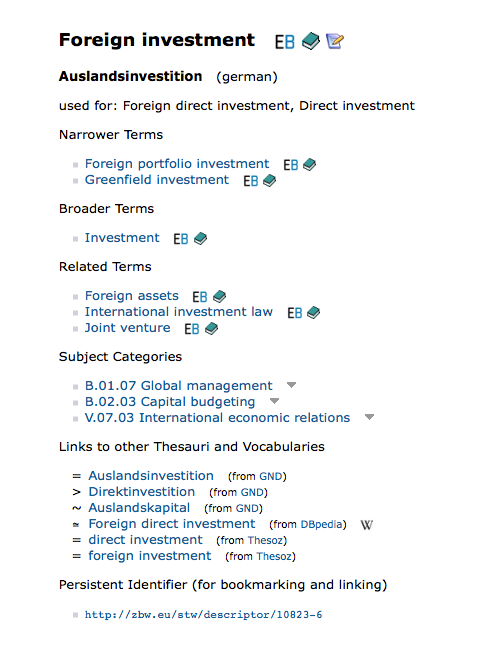
\includegraphics[height=\textheight]{zbw}};
\end{tikzpicture}
\end{frame}

\begin{frame}[plain]
\frametitle{\link{https://www.aeaweb.org/jel/guide/jel.php}{JEL codes}}
\begin{tikzpicture}
	\node at (current page.center) {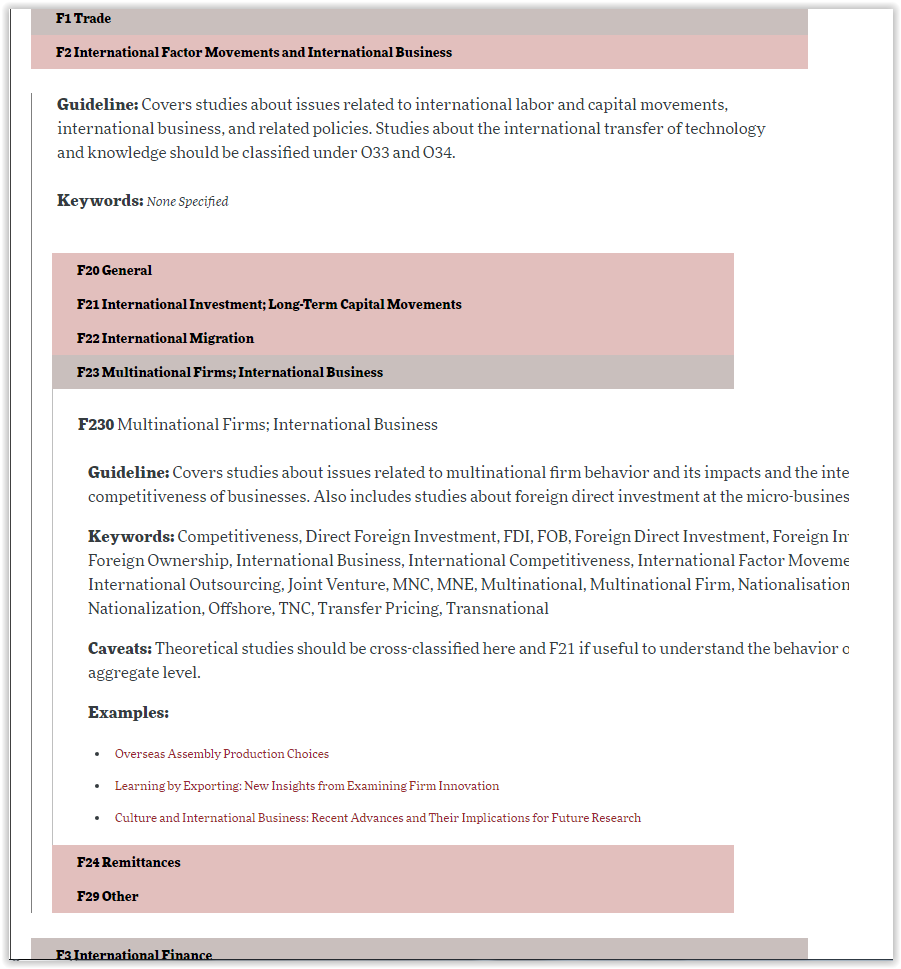
\includegraphics[width=.95\paperwidth]{JEL}};
\end{tikzpicture}
\end{frame}

\begin{frame}
\frametitle{Where to search?}
%\begin{columns}[t]
%\column{.5\textwidth}
{\color{VUBlue3}\link{https://vu.on.worldcat.org/discovery}{Libsearch}}\\
VU Library search engine, but also other collections \\
Includes books

\vfill
{\color{VUBlue3}\link{www.ubvu.vu.nl/pub/index_oclc.cfm?SearchObjectId=7&objectid=109&ordering=1&openitem=1143}{Lexis Nexis Academic}}\\
Newspapers, magazines, trade journals\\
Not very intuitive, see \link{http://libguides.vu.nl/lexisnexis-academic}{online guide} for help.

\vfill
%\column{.5\textwidth}
{\color{VUBlue3}\link{https://scholar.google.nl/}{Google Scholar}}\\
Full text search\\
Includes unpublished work!\\
Access not always clear

\vfill
{\color{VUBlue3}\link{https://vu.on.worldcat.org/oclc/60462585}{Scopus}}\\
Peer-reviewed work only\\
Many options to make search more specific

\vfill
{\color{VUBlue3}More resources \link{http://vu.on.worldcat.org/oclc/60462585}{here}}

%\end{columns}
\end{frame}

\begin{frame}
\frametitle{How to search: Forward and backward snowball}
{\color{VUBlue3}Backward snowball}\\
Which articles were used for this research?\\
Check the references in an article

\vskip 2ex

{\color{VUBlue3}Forward snowball}\\
How was this article used in other research?\\
Google Scholar / Scopus: ``Cited by: \ldots''

\vskip 2ex
{\color{FEWEB1}WARNING}\\
Useful method, but explodes quickly!

\end{frame}

\begin{frame}[plain]
    \begin{tikzpicture}[remember picture,overlay]
		\node[at=(current page.center)] (gs1a) {
			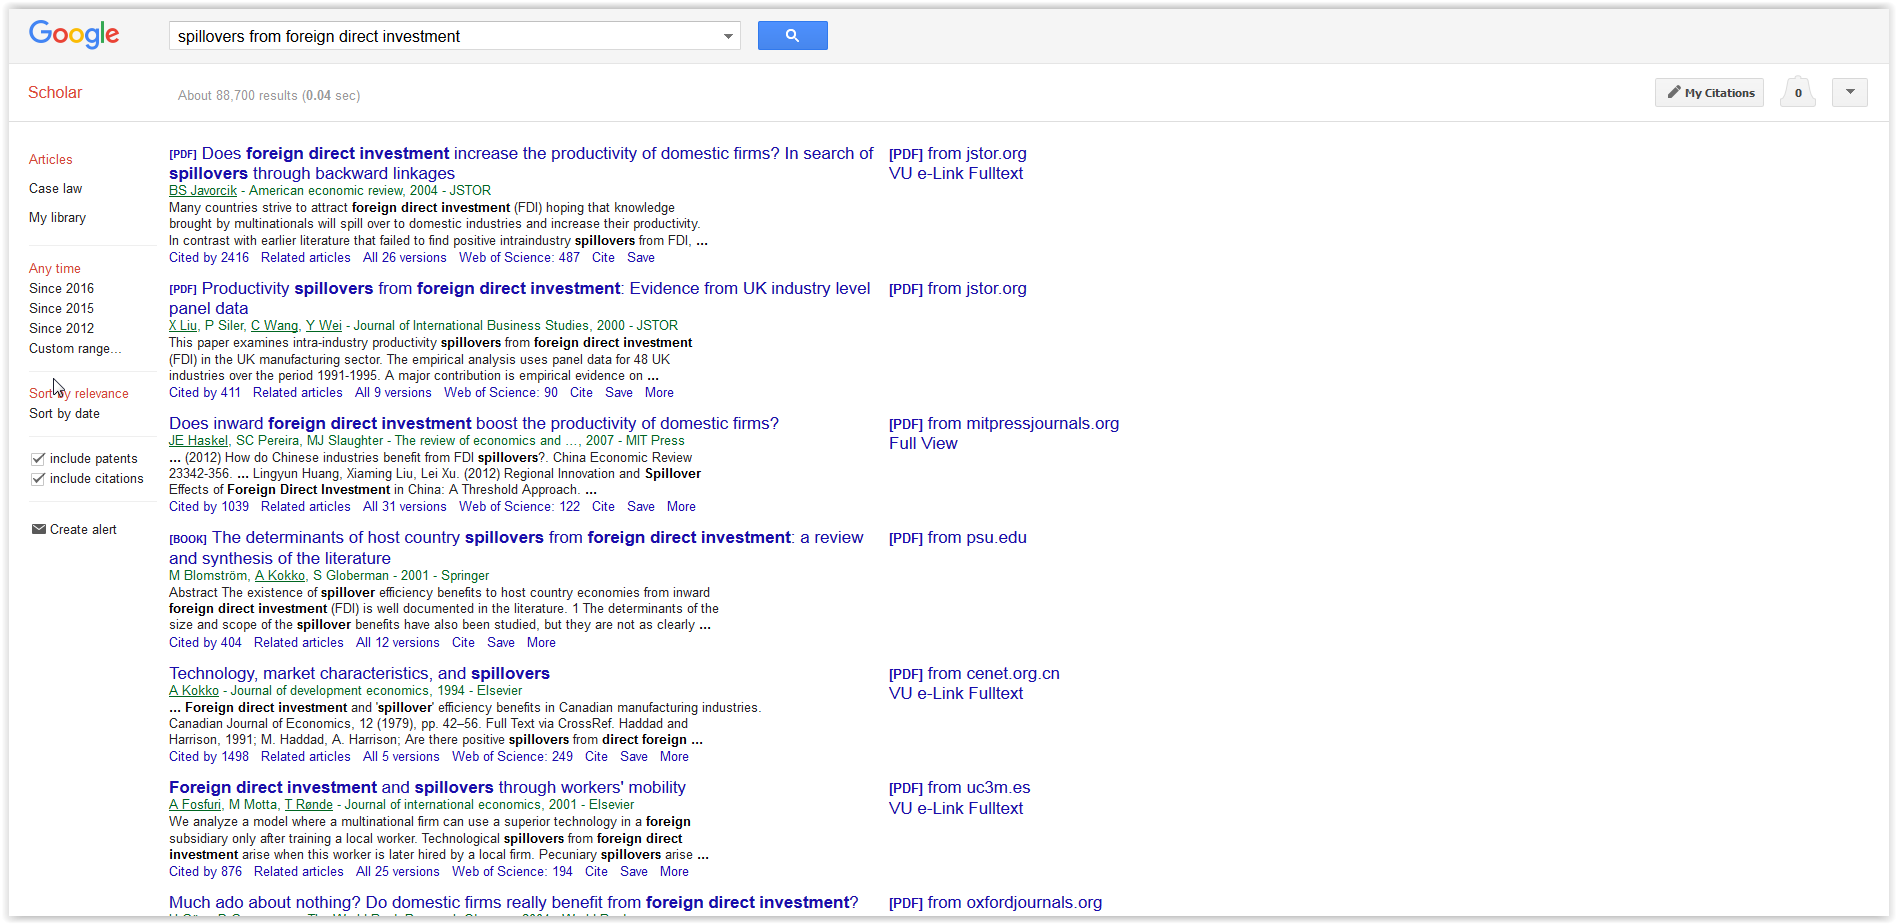
\includegraphics[width=\paperwidth]{googlescholar1a}
		};
		\only<2>{
		\node[at=(current page.center)] {
			
\includegraphics[width=.95\paperwidth]{googlescholar1b}
		};
		\path[draw, color=red, thick] (0,0.3)--(0,1.3)--(6,1.3)--(6,0.3)--cycle;
		}
	\end{tikzpicture}
\end{frame}

\begin{frame}
\frametitle{How to select articles?}
{\color{VUBlue3}Rules of thumb}
\begin{itemize}
\item Peer-reviewed work (journal articles) preferred over non-peer-reviewed (eg, working papers).\\
(Exceptions: \link{http://www.nber.org/papers.html}{NBER}, \link{http://www.iza.org/en/webcontent/publications/papers}{IZA}, \ldots)\\
\item Articles with more citations are often more influential
\item No guarantee! Use your brain first, then your advisor.
\end{itemize}
\end{frame}

\begin{frame}<1-3>[label=workflow]
\frametitle{A suggested workflow}
\begin{tikzpicture}[
	auto,%
	-{Latex[round]},%
	node distance=.5cm and .75cm,%
	shift={(current page.center)},%
	shorten <=2pt, shorten >=2pt,%
	remember picture, overlay,%
	very thick,%
	looseness=1.4,%
]
\node[rectangle, rounded corners, draw] (topic) at (-4.5cm, 3cm) {Topic search};
\node[rectangle, rounded corners, draw, below right={of topic.south}, text width=7em] (sel1) {Select, scan \&\\select again};
\node[rectangle, rounded corners, draw, below right={of sel1.south}] (snow) {Snowball search};
\node[rectangle, rounded corners, draw, below right={of snow.south}] (sel2) {Select};
\node[rectangle, rounded corners, draw, below right={of sel2.south}] (read) {Read \& select};
\node[rectangle, rounded corners, draw, below right={of read.south}] (cite) {Reference};

\draw (topic.south) to [out=-120,in=180] (sel1.west);
\draw (sel1.south) to [out=-120,in=180] (snow.west);
\draw (snow.south) to [out=-120, in=180] (sel2.west);
\draw (sel2.south) to [out=-120, in=180] (read.west);
\draw (read.south) to [out=-120, in=180] (cite.west);

\draw[dashed] (sel1.north) to [out=60,in=0] (topic.east);
\draw[dashed] (read.north) to [out=60,in=0] (snow.east);
\draw[dashed, -, shorten >=3pt] (read.north) to [out=60,in=0, curve to] node[text width=4em] {Repeat if necessary} (topic.east);

\only<2->{
\begin{scope}[on background layer, rounded corners]
	\node[fill=VUBlue2!15,fit=(topic)(sel1)] {};
\end{scope}
}
\only<3->{
\begin{scope}[on background layer, rounded corners]
	\node[fill=VUBlue2!15,fit=(snow)(sel2)] {};
\end{scope}
}
\end{tikzpicture}
\end{frame}

\section{Answering your research question}
\againframe<3>{preview}

\begin{frame}
\frametitle{Finding \& working with data}

{\color{VUBlue3}\link{http://libguides.vu.nl/finding-data}{Finding data}}\\
Important databases for company data, financial market data, economics\\
Tips for downloading data (No 1: Think before you download!)

\vskip 1ex

{\color{VUBlue3}\link{http://libguides.vu.nl/working-with-data}{Working with data}}\\
Collection of tips \& tricks:\\
Organizing data, combining data from several sources, \\
firm identifiers, event studies, \ldots

\vskip 1ex
{\color{VUBlue3}Complete list of resources \link{http://www.ubvu.vu.nl/pub/index_oclc.cfm?SearchObjectId=7&aantalitem=25&lang=&fromitem=1&max=452&ordering=1&objectid=109&trefwoord=&fctN=st3&fctIncV=13&fctExcV=+}{here}}\\
\end{frame}

\section{Communicating your answer}
\againframe<4>{preview}

\begin{frame}
\frametitle{Copy, combine, create}
{\color{VUBlue3}\link{http://quoteinvestigator.com/2013/03/06/artists-steal/}{``Good artists copy; great artists steal.''}}\\
Academics steal and leave finger prints.

\vskip 1ex
%\vfill
{\color{VUBlue3}Accountability is important}\\
What did you copy? What is your own work?\\
Plagiarism is a serious academic crime

\vskip 1ex
%\vfill
{\color{VUBlue3}Invest in automation}\\
Endnote: \link{http://download.vu.nl/}{download}, \link{http://libguides.vu.nl/endnote}{online help}\\
\link{https://www.mendeley.com}{Mendeley}\\
Integration with MS Word and others
\end{frame}

\section{More support}
\againframe<2>{titlepage}

\begin{frame}<1>[plain, label=control]
\begin{tikzpicture}[remember picture,overlay]
	\node[anchor=center, at={(current page.center)}] {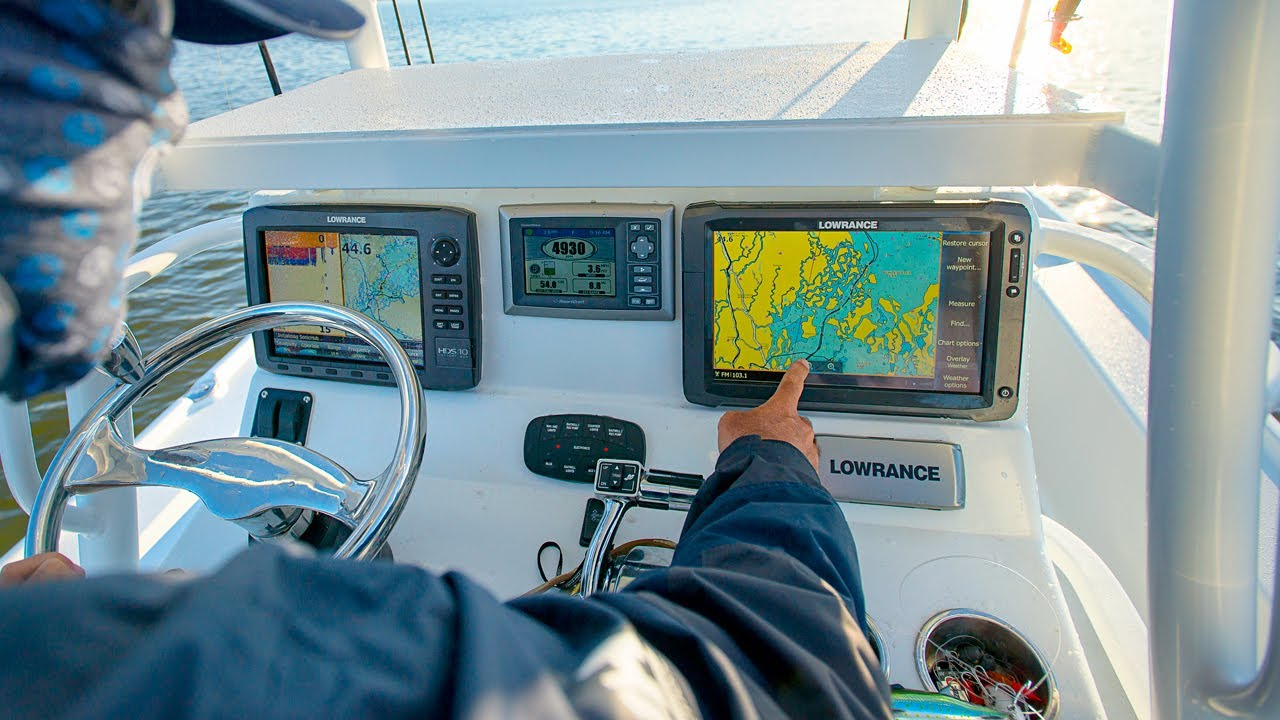
\includegraphics[width=\paperwidth]{in-control}};
\end{tikzpicture}
\only<2>{
	\begin{tikzpicture}[remember picture,overlay]
	\node at (5cm,2cm) {\LARGE\bfseries QUESTIONS?};
	\end{tikzpicture}
}
\end{frame}

\begin{frame}
\frametitle{More support}

{\color{VUBlue3}\link{http://ub.vu.nl/en/index.aspx}{Library home page}}\\
for information, opening hours, news

\vfill
{\color{VUBlue3}Relevant \link{http://libguides.vu.nl/sb.php?subject_id=109732}{online guides}}

\vfill
{\color{VUBlue3}Check the \link{http://www.ub.vu.nl/en/news-agenda/agenda/index.aspx}{Agenda}}\\
for workshops on finding literature \& data, Endnote, seminars, \ldots

\vfill
{\color{VUBlue3}\link{http://ub.vu.nl/en/education-research/research-data-services/support-for-secondary-sources/}{Research Data Services}}\\
for data questions

\vfill
{\color{VUBlue3}Info on \link{https://ub.vu.nl/en/facilities/off-campus-access/}{off-campus access}}\\

\vfill
{\color{VUBlue3}\link{mailto:vraag.ub@vu.nl}{vraag.ub@vu.nl}}\\
for questions on access, availability, \ldots

\end{frame}

\againframe<2>{control}


\end{document}
